% ############# ROZDZIAŁ 2 ###############

\chapter{Stan badań}
\label{cha:stan.badan}

W tym rozdziale postaramy się pokazać w jaki sposób badacze podchodzili do problemów powiązanych z tematem niniejszej pracy a także postaramy się rozszerzyć te podejścia.

\section{Powiązane prace – zarys historyczny}
\label{sec:zarys.historyczny}

\subsection{Predykcja wartości liczby ferrytowej}
\label{sec:liczba.ferrytowa}

Przewidywanie własności mechanicznych produktów odlewniczych za pomocą metod uczenia maszynowego ma niemal tak długą historię, jak sama dziedzina uczenia maszynowego. Już w~jednej z~pierwszych prac naukowych na ten temat \cite{Olson85} mówiono o~tym, że przyszłe techniki predykcyjne będą opierać się raczej na wyrażeniach matematycznych czy sztucznej inteligencji niż na diagramach. 
Ówcześnie do przewidywania fazy mikrostruktury spoiny metalu wykorzystywano właśnie diagramy (rys. \ref{fig:mesh1}), lecz jak łatwo się domyślić, jest to podejście mało praktyczne. Stąd nacisk na wykorzystywanie jak najbardziej wszechstronnych wyrażeń ilościowych do przewidywania mikrostruktury jako funkcji m.in. składu.

\begin{figure}[h]
    \centering
    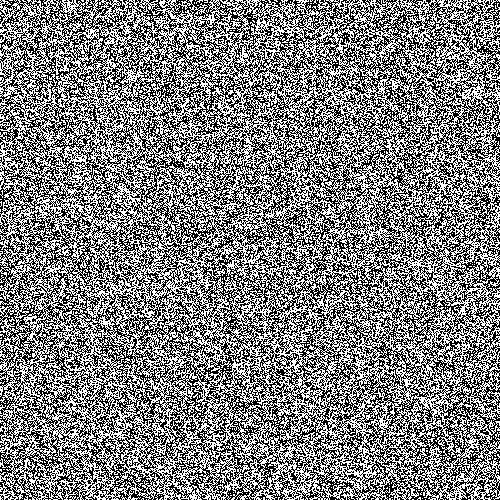
\includegraphics[width=1\textwidth]{rys.1.WRC.Delong.png}
    \caption{Przykładowy schemat do wyznaczania ferrytu $ \delta $ z~granicami składu \cite{DeLong73}}
    \label{fig:mesh1}
\end{figure}

Następnym krokiem było opracowanie modelu półempirycznego w~celu powiązania składu metalu spoiny z~liczbą ferrytową (zwaną dalej FN), czyli miarą oznaczania zawartości ferrytu w~stali nierdzewnej. Dlaczego jest to istotne? Jak wskazano w~pracy \cite{Vitek03.I} wielkość FN określa właściwości metalu, takie jak wytrzymałość, twardość, odporność na korozję i~inne (jej poziom powinien wynosić $3-7\%$, ponieważ niski poziom ferrytu może prowadzić do pęknięć \cite{ferrite.meter, Saluja15}, z~drugiej strony wysoki poziom ferrytu prowadzi do niższej odporności na korozję \cite{Saluja15}). 

W pracy Babu i~in. \cite{Babu13} przedstawiono wyniki aproksymacji punktowej, która dopasowuje model do prognoz zgodnych z~obserwacjami eksperymentalnymi. Stwierdzono w~niej, iż ogólna dokładność badanego modelu jest porównywalna do tej z~diagramu WRC-1992 (czyli najnowocześniejszej ówcześnie metody – przyp. aut.), który powstał w~ten sposób, iż skład stopu jest konwertowany do dwóch czynników – ekwiwalentu chromu ($Cr_{eq}$, wzór \ref{eq1}) oraz ekwiwalentu niklu ($Ni_{eq}$, wzór \ref{eq2}). Wynika to z~tego, iż ten pierwszy zawiera elementy, które wpływają na mikrostrukturę w~ten sam sposób jak chrom (tj. stabilizatory ferrytu), natomiast ten drugi zawiera elementy, które wpływają na mikrostrukturę w~ten sam sposób jak nikiel (tj. stabilizatory austenitu). Następnie z~diagramu można odczytać poziom ferrytu, który jest przedstawiony jako funkcja od ekwiwalentów chromu i~niklu. Jak stwierdzają autorzy \cite{Babu13}, zaletą aproksymacji punktowej w~porównaniu z~diagramem WRC-1992 jest jego zdolność do uwzględniania wpływu innych pierwiastków stopowych oraz łatwość ekstrapolacji do wyższych wartości $Cr_{eq}$ i~$Ni_{eq}$ (WRC-1992 jest pod tym względem mocno ograniczone, co widać na rysunku \ref{fig:mesh2}).
\begin{figure}[h]
    \centering
    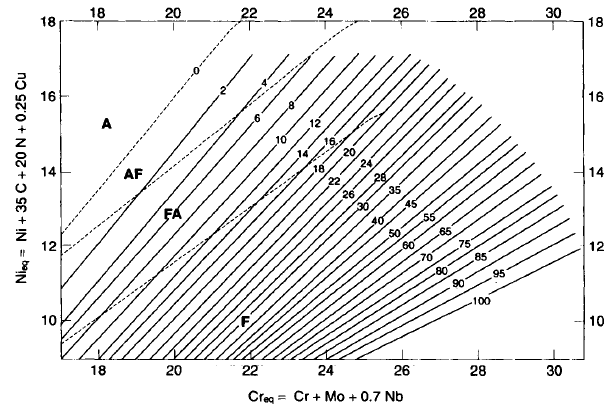
\includegraphics[width=1\textwidth]{rys.2.WRC.Kotecki.png}
    \caption{Diagram WRC-1992 \cite{Kotecki92}}
    \label{fig:mesh2}
\end{figure}

\noindent Równania na  $Cr_{eq}$ i~$Ni_{eq}$ są następujące (zgodnie z~rys. \ref{fig:mesh2}):
\begin{equation}
\label{eq1}
	Cr_{eq} = Cr + Mo + 0.7Nb
\end{equation}
\begin{equation}
\label{eq2}
	Ni_{eq} = Ni+35C+20N+0.25Cu
\end{equation}
gdzie symbole pierwiastków przedstawiają procentowy udział wagi każdego pierwiastka.
W kolejnej pracy \cite{Vitek03.I} dotyczącej predykcji FN ci sami autorzy wykorzystali sieć neuronową, która na wejściu przyjmowała procentowy udział wagi $13$ pierwiastków ($Fe$, $Cr$, $Ni$, $C$, $N$, $Mo$, $Mn$, $Si$, $Cu$, $Ti$, $Nb$, $V$~i~$Co$), czyli posiadała warstwę wejściową z~$13$ neuronami, następnie warstwę ukrytą z~sześcioma neuronami, natomiast na wyjściu był pojedynczy neuron, który zwracał liczbę ferrytową (rys. \ref{fig:mesh3}).

\begin{figure}[h]
    \centering
    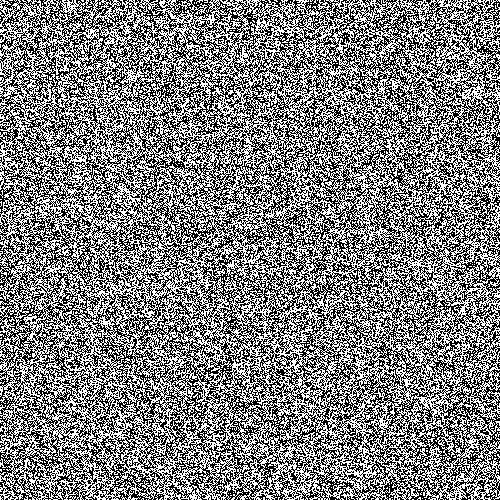
\includegraphics[width=1\textwidth]{rys.3.ORFN.Vitek.2003.png}
    \caption{Model sieci neuronowej ORFN \cite{Vitek03.I, Vitek03.II}}
    \label{fig:mesh3}
\end{figure}

Wyniki zostały przedstawione w~\cite{Vitek03.II} i~jak się okazało, testowana sieć zwracała lepsze wyniki od jakichkolwiek dotychczasowych podejść z~błędem RMS (średnia kwadratowa od ang. \textit{root mean square}) mniejszym o~$50\%$ od poprzedniej najlepszej metody. 
    W~ostatnim przytoczonym artykule dotyczącym predykcji FN \cite{Vasudevan13} również zastosowano sieć neuronową, a~konkretnie bayesowską sieć neuronową (BNN). Na wejściu mamy taką samą warstwę, jak w~poprzedniej pracy, natomiast tutaj jest więcej neuronów w~warstwie ukrytej. Poprawa wyników względem poprzedniej pracy wynosi około $15\%$ (błąd RMS) testując na niezależnym zbiorze danych nieużywanych w~szkoleniu.

\subsection{Predykcja własności mechanicznych odlewów}
\label{sub:predykcja.1}

Początki rozwoju i~przetwarzania materiałów nie były łatwe. Mimo wielu przeprowadzonych badań naukowych nad materiałami wciąż pozostaje wiele problemów, w~przypadku których brakuje metod ilościowych. Tyczy się to głównie predykcji takich parametrów konstrukcyjnych jak wytrzymałość na rozciąganie, trwałość, twardość itp. Pierwsze badania dotyczące własności mechanicznych odlewów przyjmujące podejście ilościowe brały pod uwagę szczegółowy skład chemiczny oraz takie parametry jak rekrystalizacja, proces starzenia, zakres pracy na zimno, temperatura badania czy szybkość odkształcania \cite{Bhadeshia07, Badmos13}. W~obydwu tych pracach zastosowano sieci neuronowe oraz uzasadniono, że modele matematyczne nie radzą sobie z~wymienionymi wyżej parametrami. Standardowo zastosowano sieć, w~której na wejściu podawano procent wagowy pierwiastków w~badanym materiale. 

Jedną z~głównych własności mechanicznych jest wytrzymałość na rozciąganie (ang. \textit{ultimate tensile strength}, UTS), która jest badana od wielu lat. Po fazie odlewu inżynierowie wykorzystują w~swoich obliczeniach tę i~inne wartości w~celu obliczenia odkształcania się w zależności od funkcji przyłożonego obciążenia, czasu i~wielu innych. Jest ona jednym z~ważniejszych czynników do uwzględnienia, gdyż niewystarczająca wartość wytrzymałości może mieć fatalne skutki (jak np. zawalenie się konstrukcji). Innym powodem może być to, iż jedynym sposobem na zbadanie wartości wytrzymałości jest przeprowadzenie badań niszczących, co powoduje wzrost kosztów produkcji \cite{Santos09}. Jednym ze sposobów analizy wartości UTS jest predykcja za pomocą wartości różnych właściwości odlewu. W~przywołanej wcześniej pracy \cite{Santos09} oraz \cite{Nieves09} są to skład chemiczny, rozmiar odlewu, prędkość chłodzenia, obróbka termiczna. Mając dane w~postaci wartości rozdzielonych przecinkiem (CSV, od ang. \textit{comma-separated values}) można skorzystać z~klasycznych metod klasyfikacji statystycznej, jak klasyfikacja liniowa, $k$ najbliższych sąsiadów, drzewa decyzyjne czy sieci bayesowskie \cite{wiki:klas.stat}. W~przytoczonej pracy skupiono się na sieciach bayesowskich. Wyniki są optymistyczne: dokładność na poziomie ponad 82\% oraz błędy MAE (średni błąd bezwzględny, od ang. \textit{mean absolute error}) oraz średni błąd kwadratowy (MSE, od ang. \textit{mean square error}) na poziomie odpowiednio $0.2$ oraz $0.35$. Inne przetestowane metody w~tym artykule to $k$ najbliższych sąsiadów (KNN, od ang. \textit{k-Nearest Neighbors}) oraz sztuczne sieci neuronowe (ANN, od ang. \textit{artificial neural networks}), które osiągnęły podobne, aczkolwiek nieco gorsze wyniki. 
Wytrzymałość na rozciąganie można przewidywać na podstawie dwóch różnych źródeł danych wejściowych \cite{Yang16}:
\begin{itemize}
\item
skład chemiczny metalu oraz zmienne procesu walcowania, jak temperatura, czy przebieg;
\item
dane na temat mikrostruktury. 
\end{itemize} 

\noindent W~pracy tej jako dane wejściowe wykorzystano skład chemiczny, specyfikacje geometryczne oraz zmienne dotyczące procesu rolowania, natomiast modelem użytym do predykcji wartości wytrzymałości na rozciąganie była ponownie bayesowska sieć neuronowa. Sieć ta składała się z~jednej warstwy ukrytej, która z~kolei składała się z~siedmiu neuronów. Jak stwierdzają autorzy, sieć BNN lepiej się sprawdza w~tym celu od tradycyjnych sieci neuronowych, a~to ze względu na wyższą odporność na nadmierne dopasowanie (ang. \textit{overfitting}), szczególnie w~przypadku, gdy ilość danych jest znacznie ograniczona i~nie mamy możliwości zgromadzenia dużej ilości wysokiej jakości danych.
    
Bardzo podobne podejście zastosowano w~pracy \cite{Wang20}, gdzie użyto sieci neuronowej, a~na jej wejściu podawano 20 zmiennych, takich jak skład chemiczny czy warunki obróbki cieplnej, ale również czynniki typu temperatura badania, gdyż warunku eksploatacji również mają wpływ na właściwości wytrzymałościowe. W~ten sposób uzyskano $93\%$ wartości współczynnika R-kwadrat dla granicy plastyczności (YS, od ang. \textit{yield strength}) oraz UTS.

\subsection{Predykcja błędów w~produkcji odlewniczej}
\label{sub:predykcja.2}

Innym, ciekawym podejściem jest to zaprezentowane w~pracy Penya et al. \cite{Yoseba08}, a~mianowicie ponownie zostały wykorzystane bayesowskie sieci neuronowe, lecz tym razem w~celu predykcji obecności mikrouszkodzeń w~odlewie przed lub w~trakcie procesu odlewnictwa. Dzięki takim danym można wpłynąć na proces odlewniczy w~taki sposób, aby zredukować liczbę defektów. W~sieci BNN wykorzystano na wejściu osiem zmiennych takich jak cechy geometryczne (dwie zmienne), jakość metalurgiczna (trzy zmienne), jakość formy (jedna zmienna) oraz dwie zmienne dotyczące samego procesu. Wyniki są obiecujące, gdyż dzięki temu podejściu udało się zredukować liczbę defektów z~$5\%$ do $0.075\%$ w~przypadku pierwszej odlewni oraz z~$4.7\%$ do $0.19\%$ w~przypadku drugiej odlewni.

\section{Powiązane prace – stan aktualny}
\label{sec:stan.aktualny}

\subsection{Predykcja cech i~jakości odlewów za pomocą metod rozpoznawania obrazów}
\label{sub:predykcja.3}

Wewnętrzna struktura materiału nazywana jest mikrostrukturą. Określa ona wszystkie jego właściwości fizyczne i~chemiczne. Pomimo tego, że charakterystyka mikrostrukturalna jest szeroko rozpowszechniona i~dobrze znana, klasyfikacja mikrostrukturalna jest zazwyczaj przeprowadzana „ręcznie” przez ekspertów. Ze względu na złożoność mikrostruktur (mogą się one składać z~podstruktur) ich klasyfikacja jest bardzo trudna i~dotychczas nie powstało zbyt wiele prac naukowych podejmujących się próby klasyfikacji mikrostruktur. Wcześniejsze artykuły zazwyczaj oddzielały fazę klasyfikacji mikrostruktur od fazy ekstrakcji cech \cite{Azimi18}. Dzięki postępowi metod głębokiego uczenia (ang. \textit{deep learning}, DL) otworzyły się nowe możliwości. Wiele metod głębokiego uczenia w~różnych zadaniach zwraca najlepsze wyniki, jakie udało się dotychczas uzyskać, dlatego warto się nad tymi metodami pochylić. 

W pierwszej przytoczonej tutaj pracy opracowano nową zautomatyzowaną metodę wykorzystującą dyfrakcję wstecznie rozproszonych elektronów (EBSD, od ang. \textit{electron backscatter diffraction}), aby skutecznie identyfikować i~określać ilościowo mikroskładniki ferrytowe w~złożonych mikrostrukturach różnych gatunków stali \cite{Shrestha13}. Identyfikowano rodzaj ferrytu dla każdego ziarna, co wiązało się z~powiązaną z~nimi wielkością ziaren. Różne odmiany ferrytów mają różne profile dezorientacji na granicach ziaren, aczkolwiek jest ona zależna od kąta, toteż zostało to wykorzystane w~badaniach.

Z~kolei w~pracy \cite{Britz17} zastosowano korelacyjne podejście oparte na EBSD i~mikroskopii optyczno-świetlnej (LOM, od ang. \textit{light-optical microscopy}), zamiast niezależnie korzystać z~powszechnych metod. Wykorzystując rozkład orientacji ziarna w~EBSD, ręcznie ustalono progi przy pomocy próbki referencyjnej tej samej płytki z~mikrostrukturą. Podobnie, w~przypadku LOM, próg był ręcznie ustalany i~mógł być zweryfikowany krzyżowo.

Kolejna przeanalizowana praca \cite{Azimi18} dotyczy klasyfikacji mikrostrukturalnej składników stali niskowęglowej za pomocą metod głębokiego uczenia. Takie podejście może być pomocne przy ocenie jakości danego odlewu jak i~predykcji jego właściwości mechanicznych. W~artykule wykorzystano w~pełni splotową sieć neuronową (ang. \textit{Fully Convolutional Neural Network}, FCNN), na której wejście podawano segmentowane piksele. System ten osiągnął niemal $94\%$ skuteczność, tym samym przewyższając najlepszą dotychczas metodę. Jak stwierdzają autorzy, nie tylko wynik jest doskonały sam w~sobie, ale również wyznacza linię dla przyszłych badań, m.in. związanych z~oceną jakości stali (i nie tylko). W~pracy tej, oprócz wspomnianego modelu, przetestowano również szereg innych metod oraz podejść. Jednym z~zastosowanych podziałów klasyfikacji jest klasyfikacja mikrostruktur oparta na obiekcie (ang. \textit{object-based microstructural classification}). Polega ona na wycinaniu obiektów z~obrazów, a~następnie klasyfikacji wyciętych kształtów do jednej z~kilku klas (ferryt, cementyt, austenit, perlit, bainit, martenzyt), jak pokazano na rysunku \ref{fig:mesh4}.  

\begin{figure}[h]
    \centering
    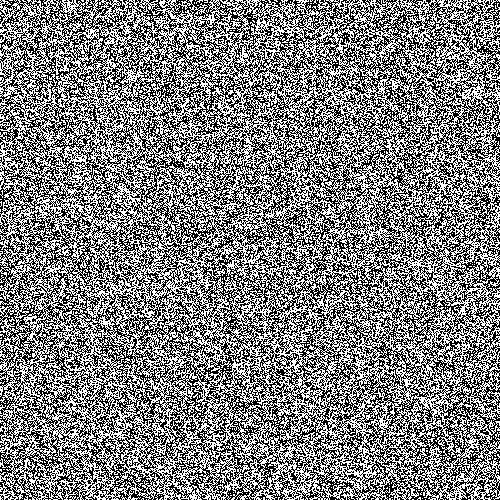
\includegraphics[width=1\textwidth]{rys.4.VGG.schema.png}
    \caption{Klasyfikacja oparta na obiektach przy użyciu CNN. Obiekty są wycinane z~obrazów a~następnie klasyfikowane przez wytrenowane CNN (VGG16). Rozmiar wejściowy jest z~góry określony \cite{Azimi18}}
    \label{fig:mesh4}
\end{figure}

\noindent Jednakże, jak zauważono w~pracy, podejście to ma jedną wielką wadę, a~mianowicie konieczna jest zmiana rozmiarów wycinanych kształtów tak, aby odpowiadała wejściu sieci neuronowej, które jest z~góry ustalone (224 na 224 pikseli). W~ten sposób możemy zniszczyć cenne dane związane np. z~teksturą. Po przeprowadzeniu testów, przy użyciu tego podejścia uzyskano wynik na poziomie 49\% dokładności (który był dotychczas najlepszy). Drugie podejście, jakie zostało przetestowane w~\cite{Azimi18} polega na klasyfikacji pod względem pikseli (rys. \ref{fig:mesh5}). Na wejście sieci są podawane obrazki, które otrzymujemy poprzez wycinanie kawałków oryginalnych obrazów metodą przesuwnego okna. Wykonujemy tę operację tyle razy, aby pokryć cały obraz wejściowy. Wyjściem takiej sieci jest macierz 3D z~liczbą kanałów równą liczbie klas. Każdy piksel tej macierzy posiada wartość reprezentującą ufność (bądź prawdopodobieństwo) przynależności do danej klasy mikrostruktury. Następnie przeprowadzany jest etap klasyfikacji według pikseli, wybierając klasę z~najwyższym prawdopodobieństwem (pewnością, ufnością) dla każdego piksela. Następnie wszystkie segmenty należące do oryginalnego obrazu wejściowego są scalane razem (rys. \ref{fig:mesh5}). Wtedy do każdego obiektu stosowana jest zasada maksymalnego głosowania i~przypisywana jest mu klasa, jaką posiada większość pikseli (tzn. obiektowi jest przypisywana klasa mikrostruktury z~maksymalną liczbą sklasyfikowanych pikseli wewnątrz obiektu). W~pracy zastosowano również równoważenie klas oraz rozszerzenie danych (ang. \textit{data augmentation}). Równoważenie klas było konieczne, ponieważ występowały duże rozbieżności pomiędzy liczebnością przykładów w~różnych klasach, natomiast oryginalne było samo podejście do tego tematu, a~mianowicie w~zależności od liczności klasy stosowano różne rozmiary kroku (ang. \textit{stride}), tak, aby uzyskać mniejszą lub większą liczbę wyciętych przykładów. Natomiast rozszerzenie danych odbyło się poprzez rotację obrazków o~90°, 180° oraz 270°, dzięki czemu zbiór obrazków został rozszerzony aż czterokrotnie. Pomimo iż sama augmentacja nie miała znaczącego wpływu na wyniki, to dzięki niej uzyskano wzrost o~2 punkty procentowe.
\begin{figure}[h]
    \centering
    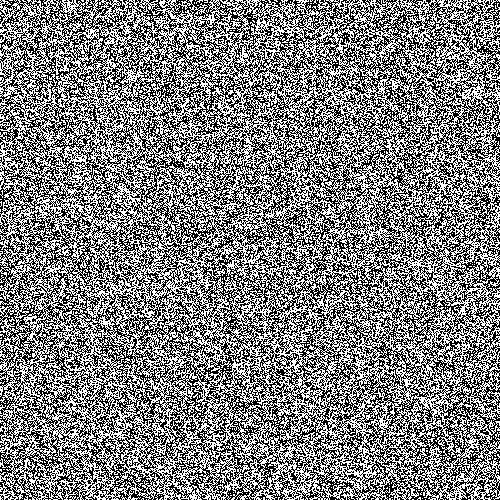
\includegraphics[width=1\textwidth]{rys.5.segmentacja.jpg}
    \caption{Klasyfikacja mikrostrukturalna oparta na segmentacji z~maksymalną liczbą głosów. Obraz wejściowy jest przycinany, wycinki są przekazywane do sieci FCNN. Następnie segmentowane wycinki są zszywane razem. W~ostatnim kroku stosowane jest głosowanie dla wynikowego zszytego obrazu \cite{Azimi18}}
    \label{fig:mesh5}
\end{figure}
Dzięki takiemu podejściu udało się poprawić najlepszy dotychczas wynik aż o~45 punktów procentowych~(sic!). Wyniki wszystkich przetestowanych metod zostały przedstawione w~tab. \ref{tab:tab1}.

\begin{table}[h]
	\centering
	\begin{threeparttable}
		\caption{Wyniki klasyfikacji mikrostrukturalnej przy użyciu metod opartych na obiektach oraz opartych na pikselach (Azimi et al., 2018)}
		\label{tab:tab1}
		\begin{tabularx}{1\textwidth}{ |X|X|X|X| }
  \hline
   \textbf{Metoda} & \textbf{Typ} & \textbf{Strategia treningu} & \textbf{Dokładność}\\
  \hline
  Pauly et al. \cite{Pauly16} & oparte na obiektach & — & 48.89\%\\
  \hline
  CIFAR-Net & oparte na obiektach & od zera (ang. \textit{from scratch}) & 57.03\%\\
  \hline
  VGG19 + SVM & oparte na obiektach & — & 64.84\%\\
  \hline
  VGG16 & oparte na obiektach & strojenie (ang. \textit{fine tuning}) & 66.50\%\\
  \hline
  MVFCNN\tnote{a} & oparte na pikselach & strojenie (ang. \textit{fine tuning} & \textbf{93.94\%}\\
  \hline
\end{tabularx}
		\begin{tablenotes}
			\footnotesize
			\item[a] Metoda MVFCNN to metoda badana w~przytoczonym artykule \cite{Azimi18}. Wynik ten został osiągnięty na obrazkach otrzymanych metodą skaningowej mikroskopii elektronowej (SEM, od ang. \textit{scanning-electron microscopy}), natomiast na obrazkach metodą LOM osiągnięto wynik zaledwie około 70\%\textellipsis
		\end{tablenotes}
	\end{threeparttable}
\end{table}

Kolejną pracą, z~obiecującymi wynikami, która również korzysta z~uczenia głębokiego, jest \cite{Durmaz21}. Celem owej pracy jest segmentacja struktur w~stali o~złożonej fazie. Autorzy zastosowali w~niej sieci Vanilla U-Net oraz U-Net VGG16, uzyskując najlepsze wyniki skuteczności odpowiednio $91.6\%$ oraz $90.6\%$. Rezultaty te otrzymano dla danych w~postaci obrazów uzyskanych metodą LOM. Wykorzystano również dane w~postaci obrazów otrzymywanych metodą SEM, lecz skuteczności były mniejsze o~około $10$ punktów procentowych.

\section{Wnioski}
\label{cha2.3}

Jak widzimy, dziedzina, jaką jest inżynieria materiałowa, mimo iż rozwijana już od wielu lat, nadal wymaga wiele pracy, która usprawni proces wytwarzania materiałów, a~także zaoszczędzi środki, które obecnie są marnowane na badania niszczące. Właściwości materiału takie jak wytrzymałość, wiązkość, twardość, kruchość lub ciągliwość są istotne przy kategoryzacji materiału lub komponentu według ich jakości, lecz testy te są zwyczajowo drogie. Dlatego metody uczenia maszynowego są uznawane za pomocne w~przewidywaniu właściwości odlewów \cite{Stoll21}. Z~drugiej strony problemem może być wciąż niewystarczająca ilość danych uczących –  co można zauważyć po tym, iż nie udało się znaleźć żadnych publicznie udostępnionych danych w~postaci zdjęć, które można byłoby dołączyć do własnego zbioru danych. Z~tego też względu przeprowadzone testy będą się opierały głównie na klasyfikacji metalu ze względu na wysoką bądź niską odporność na rozciąganie, a~także ze względu na wysoką bądź niską granicę sprężystości, gdyż takimi właśnie danymi dysponujemy.

Początkowo w~celu predykcji właściwości mechanicznych korzystano z~dosyć prymitywnych rozwiązań jak np. odczytywanie z~wykresu właściwości za pomocą samego składu chemicznego. Następnie, po wielu latach rozwoju w~dziedzinie materiałoznawstwa, jak i~informatyki i~uczenia maszynowego zaczęto korzystać z~takich zmiennych jak skład chemiczny, wielkość odlewu, prędkość chłodzenia czy proces obróbki termicznej wykorzystując takie modele, jak sieci bayesowskie, algorytm k-nn czy sieci neuronowe. Z~czasem sieci neuronowe zaczęły osiągać najlepsze wyniki, w~tym momencie znacznie zostawiając w~tyle pozostałe metody. A~więc co do wykrywania właściwości mając wspomniane wcześniej dane, sieci neuronowe zostały dosyć dobrze przetestowane i~dają gwarantowane, wysokie wyniki. Co natomiast z~danymi w~postaci obrazów? Tutaj widzimy, że powoli również są adaptowane sieci neuronowe, a~w~szczególności głębokie sieci neuronowe \cite{Azimi18, Pauly16}, które dają nadzwyczaj obiecujące wyniki. Natomiast prace te były związane z~wykrywaniem pojedynczych struktur na obrazkach, a~nie z~predykcją samych właściwości mechanicznych. Wykorzystano w~nich tzw. semantyczną segmentację obrazu, która wydaje się najbardziej optymistyczna, aczkolwiek nie posiadamy takich danych. Jednak jak najbardziej można to uznać za obiecujący kierunek poszukiwań w~celu zwiększenia skuteczności sieci wykrywających i~klasyfikujących struktury na obrazkach.

Podsumowując, sieci neuronowe udowodniły swoją przydatność w~zakresie predykcji zawartości ferrytu w~składzie chemicznym spoiny czy predykcji właściwości mechanicznych za pomocą składu chemicznego i~danych dotyczących samego procesu wyrobu takiego materiału. Znaczące postępy też są widoczne w~obszarze klasyfikacji struktur na obrazie. Jednak nadal brakuje badań w~obszarze predykcji właściwości mechanicznych z~obrazów, dlatego autor niniejszej pracy podjął się próby przeprowadzenia takich testów i~przeanalizowania możliwości sieci neuronowych (w szczególności głębokich sieci neuronowych) w~tym zakresie. Dysponując oznakowanymi danymi w~postaci obrazków, które zostały podzielone na dwa podzbiory –  ze względu na odporność na rozciąganie oraz ze względu na granicę sprężystości, warto przetestować możliwości predykcyjne sieci neuronowych dla tak postawionego problemu. Dodatkowo można skorzystać z~pomysłów (przedstawionych w~powyższych podrozdziałach) dotyczących klasyfikacji struktur na obrazach, aby mieć dodatkowe informacje, które być może będą pomocne w~docelowej klasyfikacji. Oprócz tego, jako inne źródła informacji można z~obrazów wyciągać momenty, które zostały opracowane wiele lat temu i~dotychczas były wykorzystywane z~sukcesami. Ponadto, głównie jako odniesienie, można wykorzystać klasyczne klasyfikatory typu las losowy, maszyna wektorów nośnych czy inne. Oczekuje się wyników na poziomie zbliżonym do wyników przedstawionych w~powyższych pracach, które korzystały z~sieci neuronowych dla danych zawierających m.in. skład chemiczny.  







